
\section{Background and Related Work}
\subsection{The PageRank Algorithm}
% Describe how PageRank works: power iteration, damping factor, convergence.

\begin{itemize}
  \item explain PageRank in 2 sentences
  \item history of the algorithm
  \item how does it work? 
  \item explain different methods of PageRank (Pregel in GraphX, Approxminate PR, ...)
  \item applications of PageRank
\end{itemize}

PageRank is an algorithm originally introduced to measure a website's relevance on the World Wide Web. A website's rank is higher the more websites link to it. It was created by Larry Page and Sergey Brin, the founders of Google, to optimize the search engine.
The foundation of the algorithm is a graph where every node represents a website in the internet and an edge translates to a hyperlink on a website.
\begin{figure}[ht]
    \centering
    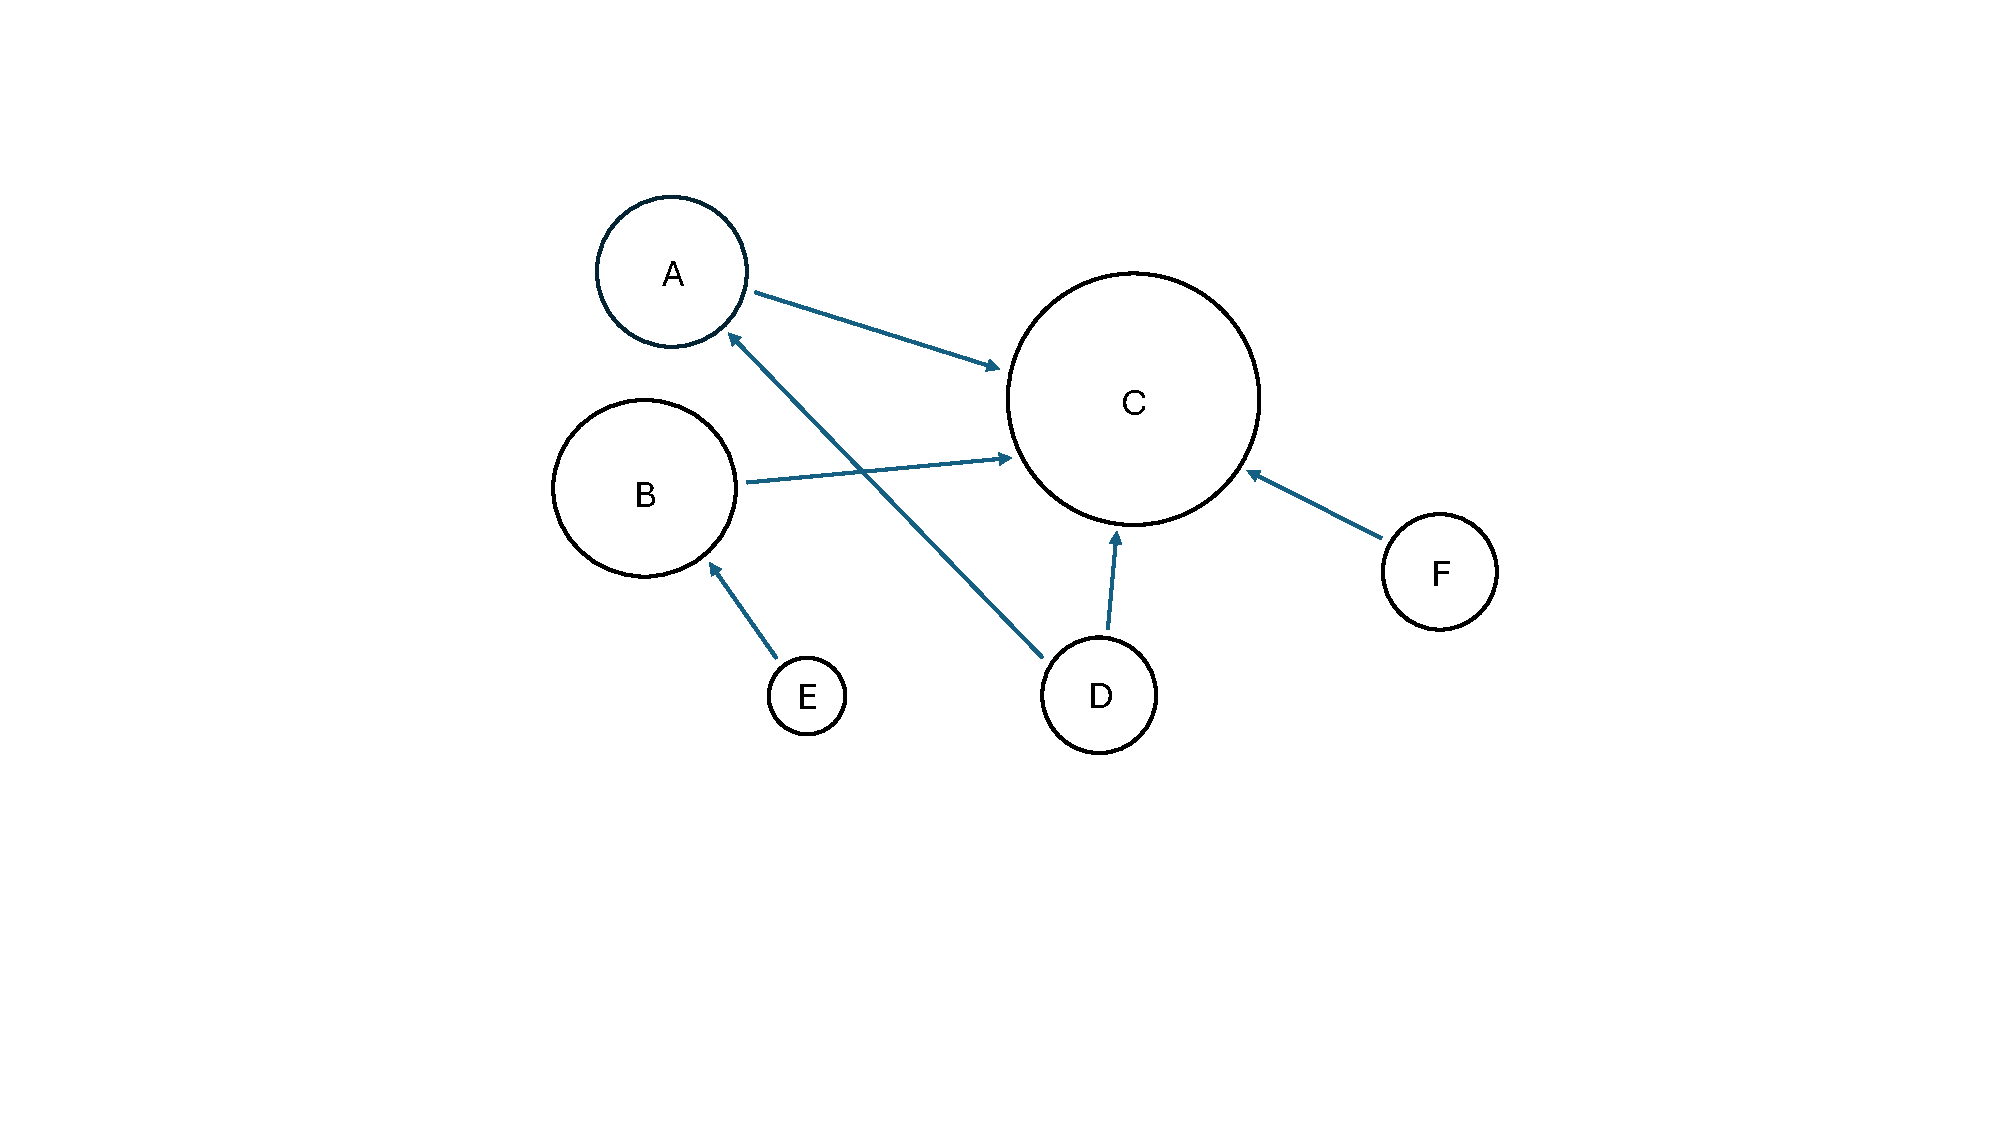
\includegraphics[width=0.7\linewidth]{images/PageRank Graph.pdf}
    \caption{PageRank Graph}
    \label{fig:pagerank-toy}
\end{figure}

To calculate the PageRank values, a transition matrix is constructed, in which each row represents a state, a website, and contains the probabilities of moving from one node to another. In figure 1 D has two outgoing edges, so the probability of moving from D to another node is $0.5$. The transition matrix describes the behavior of a "random surfer". The random surfer model describes the probability of a random user visiting a website. Finding the PageRank values is a Markov chain process, and its stationary distribution is the PageRank vector. Additionally, to model realistic user behavior, a damping factor is introduced, which is commonly set to 0.85. That means with probability $\alpha$ a random surfer clicks on an outgoing hyperlink on the current website and with probability $1-\alpha$ the surfer "teleports" to a random website in the graph. This characteristic is necessary for PageRank because web graphs can have dangling nodes, disconnected parts or cycles. Thus, the damping factor ensures that the Markov chain is irreducible and aperiodic, which guarantees a convergence to a unique stationary distribution. 
The PageRank algorithm is commonly defined as the following:
\begin{equation}
    \pi_v = \frac{1-\alpha}{n}+c\sum_{u\in N^-(v)}\frac{\pi_u}{d^+(u)} \quad\text{\cite{chebolu_pagerank_2008},}
\end{equation} 
where: 
\begin{itemize}
    \item $\pi_v$ is the PageRank of the node $v$
    \item $\alpha$ is the damping factor
    \item $n$ is the total number of nodes in the graph
    \item $N^-(v)$ is the set of ingoing edges of $v$
    \item $d^+(u)$ is the out degree of $u$
\end{itemize} 
% talk about tolerance and convergence
The calculation of PageRank follows the power iteration method, a technique to finding the dominant eigenvalue. The iterative process is defined as follows
\begin{enumerate}
    \item Define the initial vector 
    \begin{equation}
        \pi^{(0)}=\frac{1}{n}e
    \end{equation}
    \item At each iteration apply the update rule, where $S$ is the transition matrix and $e$ is the all-ones vector
    \begin{equation}
        \pi^{(k+1)} = \alpha S^T+ \frac{(1-\alpha)}{n}e
    \end{equation}
    \item Continue until the difference between iterations is less than a tolerance $\epsilon$
    \begin{equation}
        ||\pi^{(k+1)}-\pi^{(k)}||_1<\epsilon \quad \text{\cite{langville_googles_2012}\cite{page_pagerank_1999}}
    \end{equation}
    
\end{enumerate}
Then $\pi$ satisfies 
\begin{equation}
    \pi=G^T\pi, \quad \text{where $G=\alpha S +\frac{1-\alpha}{n}ee^T$}
\end{equation}
and $\pi$ is a stationary probability distribution, the unique PageRank vector.
Each entry in the PageRank vector represents the probability that a random surfer will land on a specific node. The power iteration method has a time complexity of $O(m)$ per iteration, where $m$ is the the number of edges. Thus, the total complexity is $O(m\cdot k)$. The number of iterations $k$ depends on the damping factor ,$\alpha$, and the tolerance ,$\epsilon$.

 
\subsection{Challenges in Large-scale Graph Processing}
% Memory and computational bottlenecks with big graphs.
\begin{itemize}
  \item also take parts of the introduction
\end{itemize}

\subsection{Apache Spark and GraphX}
% Explain architecture, vertex-centric computation, and limits of GraphX PageRank.
\begin{itemize}
    \item explain apache spark and graphx architecture
    \item explain memory management
    \item explain PageRank algorithm of GraphX
    \item explain RDD's
\end{itemize}

\subsection{Approximate PageRank Methods}
% Iteration, sampling, matrix approximation, and Monte Carlo approaches.
\begin{itemize}
    \item explain approximate pagerank methods also take parts of introduction
    \item explain how it's more memory efficient than original methods
\end{itemize}